\documentclass[12pt]{article}
\usepackage[hungarian]{babel}
\selectlanguage{hungarian}
\usepackage[utf8]{inputenc}
\usepackage[T1]{fontenc}

\pdfpageheight\paperheight
\pdfpagewidth\paperwidth
\setlength\topmargin{-1cm} \setlength\oddsidemargin{-0cm}
\setlength\textheight{25cm} \setlength\textwidth{15.8cm}
\setlength\columnsep{0.25in}  \newlength\titlebox \setlength\titlebox{2.00in}
\setlength\headheight{5pt}   \setlength\headsep{0pt}
\setlength\footskip{1cm}
\setlength\leftmargin{0.0in}

\usepackage{alltt}

\usepackage{tikz}
\usetikzlibrary{shapes,shapes.geometric,shapes.multipart,calc}

\usepackage{subfig}
\date{}
\title{5. gyakorlat -- Bináris és binomiális kupacok}
\begin{document}

\maketitle

\noindent 1. Hajtsuk végre a {\scshape Sorba()} műveletet egy üres maximum 
kupacon a következő elemekkel: 3, 8, 2, 11, 20, 4, 6, 9.
Mi lesz a {\scshape Sorbol()} eredménye?

A {\scshape Sorbol()} művelet a gyökérelemet törli, melynek helyét 
a kupac ``tömbös'' reprezentációja szerinti legmagasabb indexű eleme veszi át, 
majd kulcscserékkel helyreállítunk.

\begin{figure}[!ht]
\centering
\subfloat[{\scshape Sorba()} műveletek után]{
	\begin{tikzpicture}[-,thick,every node/.style={shape=circle,inner 
	sep=1pt,draw,thick,minimum width=.6cm}]
		\node {20}
			child[sibling distance=3cm]{ node {11}
				child[sibling distance=2cm]{ node {9}
					child{ node {3}}
					child[missing]
				}
				child[sibling distance=2cm]{ node {8}}
			}
			child[sibling distance=3cm]{ node {6}
				child[sibling distance=2cm]{ node {2}}
				child[sibling distance=2cm]{ node {4}}
		};
	\end{tikzpicture}
} \hfil
\subfloat[{\scshape Sorbol()} művelet után]{
	\begin{tikzpicture}
        [-,thick,every node/.style={shape=circle,inner 
        sep=1pt,draw,thick,minimum width=.6cm}]
		\node  {11}
			child[sibling distance=3cm,level distance=2cm]{ node {9}
				child[sibling distance=2cm]{ node {3}}
				child[sibling distance=2cm]{ node {8}}
			}
		child[sibling distance=3cm,level distance=2cm]{ node {6}
			child[sibling distance=2cm]{ node {2}}
			child[sibling distance=2cm]{ node {4}}
		};
	\end{tikzpicture}
}
\end{figure}


\vspace{.5cm}

\noindent 2. Egyesítsük az alábbi két minimális binomiális kupacot.
        \begin{figure}[!ht]
        \centering
        \subfloat[]{
        \begin{tikzpicture}
        [-,thick,every node/.style={shape=circle,inner 
        sep=1pt,draw,thick,minimum width=0.6cm}]
        \node (a) at (0,0) {9};
        %%
        \node (b) at (2,0) {7}
          child {node {14}
            child {node at (0,0) {21}}
          }
          child {node at (-.75,0) {11}
          }
        ;
        \path
        \foreach \startNode/\endNode in {a/b}
        {
          (\startNode) edge[-,thick] (\endNode)
        };
        \end{tikzpicture}
        } \hfil
        \subfloat[]{
        \begin{tikzpicture}
        [-,thick,every node/.style={shape=circle,inner 
        sep=1pt,draw,thick,minimum width=0.6cm}]
        \node (a) at (0,0) {6};
        %%
        \node (b) at (2,0) {10}
          child {node {12}};
        %%
        \node (c) at (4,0) {1}
          child {node {4}
            child {node at (0,0) {12}}
          }
          child {node at (-.75,0) {23}
          }
        ;
        \path
        \foreach \startNode/\endNode in {a/b, b/c}
        {
          (\startNode) edge[-,thick] (\endNode)
        };
        \end{tikzpicture}
        }
        \end{figure}

\end{document}